\frame{
    \frametitle{Evaluating retention order prediction}

% \begin{small}

\begin{block}{Dataset and molecule representation}
\begin{itemize}
    \item 1098 retention times of 946 unique molecular structures
    \item 5 different reversed phase LC-systems (denoted with $\hat{S}$)
%     \item We use counting MACCS dictionary fingerprints with MinMax-Kernel \cite{Ralaivola2005}.
    \item Molecules represented using counting MACCS fingerprints:
    
\begin{center}
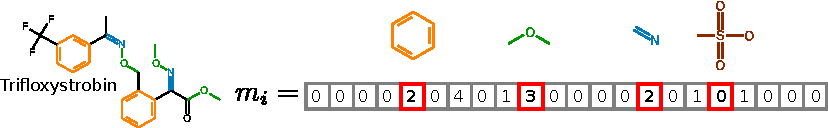
\includegraphics[scale=0.6]{images/count_fingerprints_example.pdf}
\end{center}
\vspace{-0.5cm}    
    %with MinMax-Kernel \cite{Ralaivola2005}.
\end{itemize}
\end{block}
\begin{block}{Evaluation measure and protocol}
\begin{itemize}
    \item Pairwise prediction accuracy for a target system $\sys\in\hat{S}$:
\begin{equation}
    Acc(s)\equiv\frac{|\{(i,j)\in\Pref(s)\,|\,\VEC{w}^T\phi(\mol_i)<\VEC{w}^T\phi(\mol_j)\}|}{\Pref(s)}
\end{equation}
\vspace{-0.5cm}
    \item Accuracy accessed using repeated 10-fold cross-validation.
%     \item no test molecular structure in the training set
\end{itemize}
\end{block}
% \end{small}
}



\frame{
    \frametitle{Train model with preferences from different systems}
    \framesubtitle{Can pairwise predictor benefit from information of different systems?}

\begin{block}{Compare performance of different training sets}
\begin{itemize}
    \item Single system, target data only: $\Pref(\sys)$
    \item Multiple systems, \emph{no} target data: $\Pref\setminus\Pref(\sys)$
    \item Multiple systems, all available data: $\Pref$
    \item Varying percentage of target system molecules used for training
\end{itemize}
\vspace{-0.25cm}
\end{block}
\begin{block}{Comparison method}
\begin{itemize}
    \item Support Vector Regression (SVR) trained on retention times directly \cite{Aicheler2015}.
    \item Multiple systems: Retention times are considered jointly.
\end{itemize}
\end{block}
}

\frame{
    \frametitle{Train model with preferences from different systems}
    \framesubtitle{Application setting: Training retention times only available from single target system.}
    
\begin{center}
    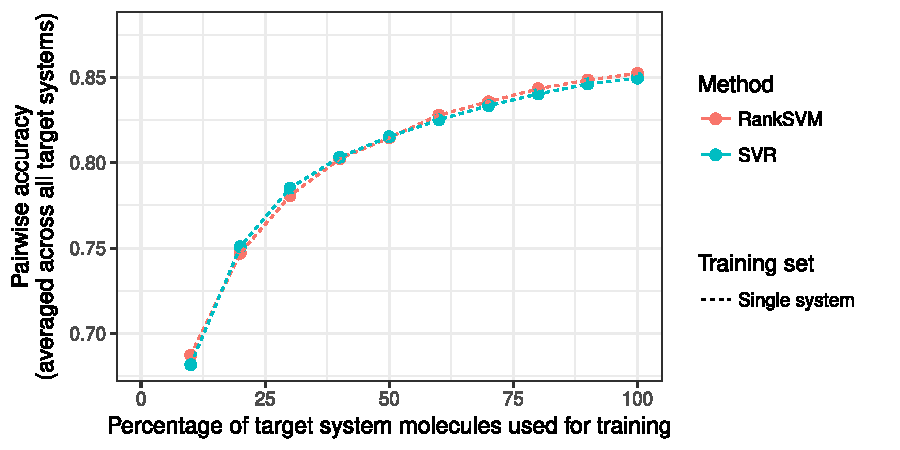
\includegraphics[width=0.9\textwidth]{images/pwacc_2_only_single_system.pdf}
\end{center}
\vspace{-0.25cm}
\begin{block}{Observations}
\begin{itemize}
    \item Increasing amount of training data improves prediction.
    \item RankSVM and SVR perform equally.
\end{itemize}
\end{block}
}

\frame{
    \frametitle{Train model with preferences from different systems}
    \framesubtitle{Application Setting: Training retention times only available \emph{from not target} system.}
    
\begin{center}
    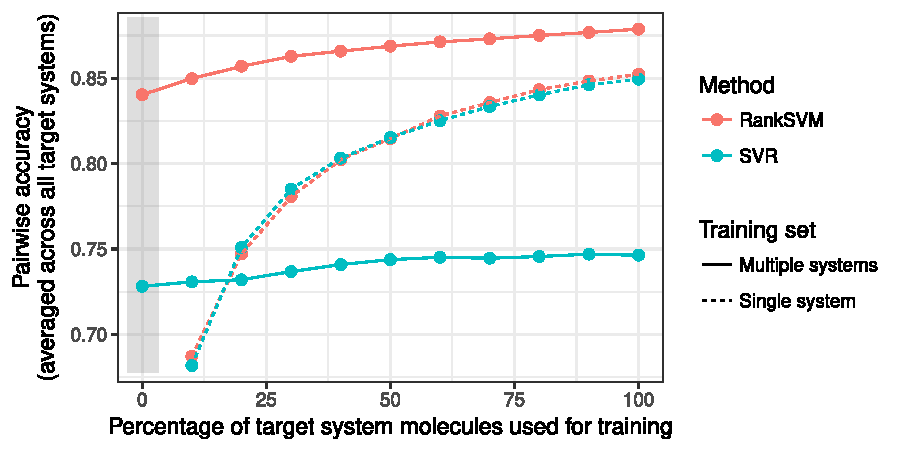
\includegraphics[width=0.9\textwidth]{images/pwacc_2_multiple_system_1.pdf}
\end{center}
\vspace{-0.25cm}
\begin{block}{Observations}
\begin{itemize}
    \item Performance of single system \emph{without} data from the target. 
    \item RankSVM outperforms SVR by considering retention \emph{orders}.
\end{itemize}
\end{block}
}
 
\frame{
    \frametitle{Train model with preferences from different systems}  
    \framesubtitle{Application Setting: Training retention times from target \emph{and} others systems available.}
    
\begin{center}
    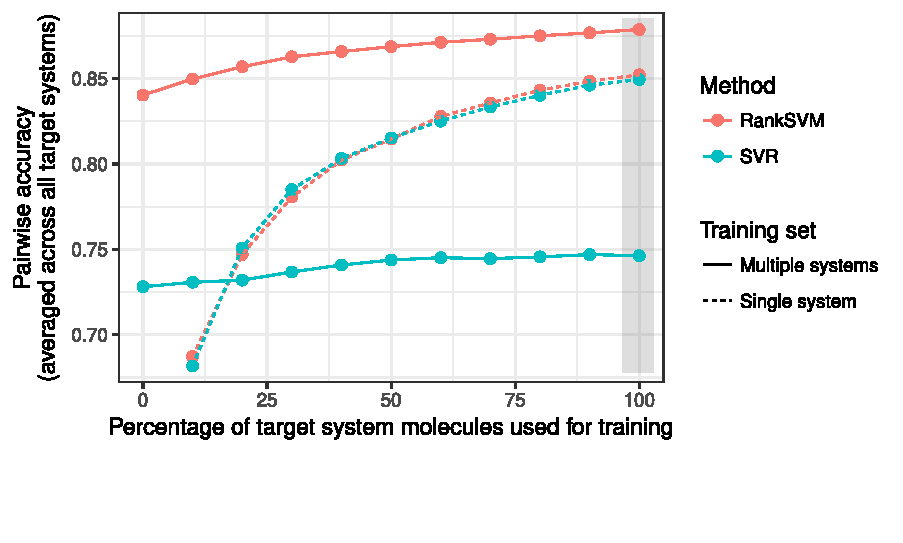
\includegraphics[width=0.9\textwidth]{images/pwacc_2_multiple_system_2.pdf}
\end{center}
\vspace{-0.25cm}
\begin{small}
\begin{block}{Observations}
\vspace{-0.15cm}
\begin{itemize}
    \item Considering target \emph{and} non-target systems' data outperforms single system.
    \item RankSVM again outperforms SVR.
\end{itemize}
\end{block}
\end{small}
}
